%\section{Thrust 2.  API Usage Code Synthesis: Models, Representations, and Methodologies}

\section{Plan-to-Do: Design Framework and Environment for Code Representation Learning}
\label{thrust2:sec}

\subsection{T1 Task 1. Conceptual Design Framework for Code Representation Learning}
This task is to propose a conceptual CRL framework abstracted and
summarized from our practical design experience to help design an
effective and accurate CRL under the context of bug detect-fix
processes.

%Let us illustrate a manual process of designing a code
%representation learning to motivate this task.

\textbf{Illustrating Example}. To detect a bug, we need to model
methods and their relations into code vectors.  To have a proper CRL,
we need to make several key design choices: (Choice
\textbf{C\circled{1}}), we need to have a code representation for a
method. A method can be represented in multiple ways, such as a bag of
AST paths, an AST, a sequence of all tokens in the method,
etc. (Choice \textbf{C\circled{2}}), we need to choose an embedding
technique for a chosen representation.  There can be at least several
well-known embedding techniques: word2vec, one-hot encoding, and
user-defined vocabulary encoding, etc.
%Taking \textit{a bag of AST paths} to represent a method as an
%example, for each path of AST nodes, we can treat each AST node as a
%word and use word2vec to generate an embedding vector for each
%node. Now,
If we use paths, a path can be represented as an ordered list of node
vectors.  (Choice \textbf{C\circled{3}}), to generate only one vector
for a path (a path vector), we need to choose a way to combine all
node vectors.  There can be many ways to convert a set of vectors into
one vector (i.e., reducing dimensions), such as using RNN, simply
concatenating all node vectors, and using a set of fully connected
layers in~\cnn.  (Choice \textbf{C\circled{4}}), now a method can be
represented as a set of path vectors. To learn a vector for a method,
we need to choose a way to combine path vectors into one method
vector.  (Choice \textbf{C\circled{5}}), once we have method vectors
for all methods in a project, we need to choose the code
representations that can capture relations among methods, such as
method-call graph and PDG.  (Choice \textbf{C\circled{6}}), we need to
choose embedding techniques and learning models to capture the
relations among methods and add them into a method vector. Here, a
method vector models two types of information: the method body and its
relations with other methods. To test a simple idea of capturing
relations among methods, we have made \textit{a set of choices}
{\textbf{C\circled{1}},\textbf{C\circled{2}},\textbf{C\circled{3}},
  \textbf{C\circled{4}}, \textbf{C\circled{5}}, \textbf{C\circled{6}}}
to generate a proper vector for a method. \textbf{Our initial
  conceptual framework} defines a list of building blocks and
guidelines (Table~\ref{framework}):

%Last, we can run a classification model on the generated method
%vectors to train a classification model to judge whether a given
%method buggy or non-buggy.

%{\color{red}{Choice C3, the last sentence, it is often called fully connection layer instead of full connected layer. I am not sure if it is a small problem.}}

%Designing a CRL approach requires the knowledge from both SE/PL and
%deep learning research fields, and importantly, the design of a code
%representation learning can be complex and requires some design
%debugging.  Our proposed framework can be very useful to provide
%guidelines for researchers to build their own code representation
%learning.


\begin{table}[h]
	\vspace{-15pt}
	
	
	\begin{center}
		%\renewcommand{\arraystretch}{1}
		\footnotesize{
			\caption{Building Blocks and Design Guidelines. A list of blocks is not an exhausted list.}\label{framework}
			\vspace{-10pt}
		%	\begin{tabular}{p{6.5cm}<{\centering\raggedright}|p{10cm}<{\centering\raggedright}}
		\begin{tabular}{p{16.5cm}<{\centering\raggedright}}
				
				\hline
			\textbf{Blocks} and \textbf{\textit{Explanation}} and \textbf{Examples}\\
				\hline
				
			\textbf{Code Representations}: \textit{Data structures representing software entities}. \textbf{Examples}: Identifiers, sequences of tokens at statement and method -level, Program Dependency Graph (PDG) at method and project -level, Control-Flow Graph (CFG), Data-Flow Graph (DFG), Abstract Syntax Tree (AST), Paths in AST, sub-AST at statement-level, Paths in PDG at method-level, Paths in CFG and DFG, Class Dependency Graph, execution paths of statements, intermediate representations.\\
				\hline
			\textbf{Relations}: \textit{Modeling relations among entities}. 
			\textbf{Examples}: Sequential relations among tokens in a statement (or a whole method), sequential relations among AST nodes in an AST path, 			sequential relations among statements in a PDG path, sequential relations among statements, relations between code and testing information, relations among test cases.  \\
				\hline
			\textbf{Embeddings}: \textit{Techniques directly encoding raw code into vectors}. 
			\textbf{Examples}: one-hot encoding, word2vec~\cite{word2vec} and Glove~\cite{Glovepennington2014glove} modeling sequential relations among words, WordMoverDistance~\cite{huang2016supervised}, vocabulary-based encoding (e..g, identifier-based, key concepts extracted from a method), ELMo~\cite{peters2019knowledge}, CoVe~\cite{mccann2017learned}, BERT~\cite{devlin2018bert} and GPT~\cite{GPTradford2018improvingGPT} for contextual word embeddings, Tree-LSTM~\cite{Tai-2015} for encoding a tree structure, Node2Vec~\cite{Grover-2016} and DeepWalk~\cite{perozzi2014deepwalk} for encoding nodes a graph.\\
				\hline
			\textbf{Learning Models}: \textit{Learning techniques taking vectors as inputs. The vectors can be initially obtained from Embedding techniques}. \textbf{Examples}: LSTM~\cite{hochreiter1997long}, GRU~\cite{Cho-2014}, HMRNN~\cite{chung2016hierarchical}, basic CNN, H-CNN~\cite{gao2018hierarchical}, R-CNN~\cite{girshick2015region}, Densely-CNN~\cite{wang2018densely}, fully connected layers in~\cnn, multi-head attention~\cite{Vaswani-2017}, MLP~\cite{bourlard1988auto}\\
			\hline
			
		%	Connecting Vectors & Techniques combining multi-vectors (2 or more) into one vector. &LSTM~\cite{}, GRU~\cite{}, HMRNN~\cite{}, basic CNN, H-CNN~\cite{}, R-CNN~\cite{}, Densely-CNN~\cite{}, fully connected layers, multi-head attention, MLP\\
		%	\hline
			
			\textbf{Existing CRLs}: \textit{A CRL takes code and learns vectors to represent the code. A CRL can be built on several code representations, Embeddings, and learning models}. \textbf{Examples}: DeepSim\cite{Zhao-2018}, code2vec\cite{Alon-2018}, Code Vectors \cite{Henkel-2018}, Deep Learning Similarity\cite{Tufano-2018}, Tree-based LSTM \cite{Tai-2015}, Ratchet\cite{Rachet}, Tufano et al. (2018)\cite{tufano2018empirical}, CODIT\cite{CODIT}, Tufano et al.~\cite{Tufano}, DeepFL\cite{DeepFL}, cuBERT~\cite{kanade2020learning}.\\
			\hline
			
		    \textbf{Design Principles}: \textit{Empirically obtained best practices and design rules}. \textbf{Examples}: LSTM is not good for combining vectors from different information sources, but multi-head attention is designed for combining multiple vectors from distinct sources.\\
			\hline
			
			\end{tabular}
			%~(P: the probability of generated plausible patches to be correct)
		}
		
	\end{center}
	\vspace{-15pt}
\end{table}

	


\subsection{T1 Task 2. Designing A Visual Design Environment to Support Code Representation Learning}

We design a visual editing environment to support CRL framework.
Our editor design has the following components (Figure~\ref{editor}): \underline{{\em (1) Code
    Representations}:} shows a list of pre-defined code
representations, e.g., the ones in the row ``Code Representations'' of
Table~\ref{framework} and a user-defined data structure (if users
upload their data structures).  \underline{\textit{(2) Embeddings:}}
shows a list of approaches for encoding representations, e.g., the
ones in the row ``Embeddings'' of Table~\ref{framework} and a
user-defined embedding (if users upload the encoded vectors).

 \begin{wrapfigure}{r}{0.75\textwidth}
	\centering
	\vspace{-10pt}
	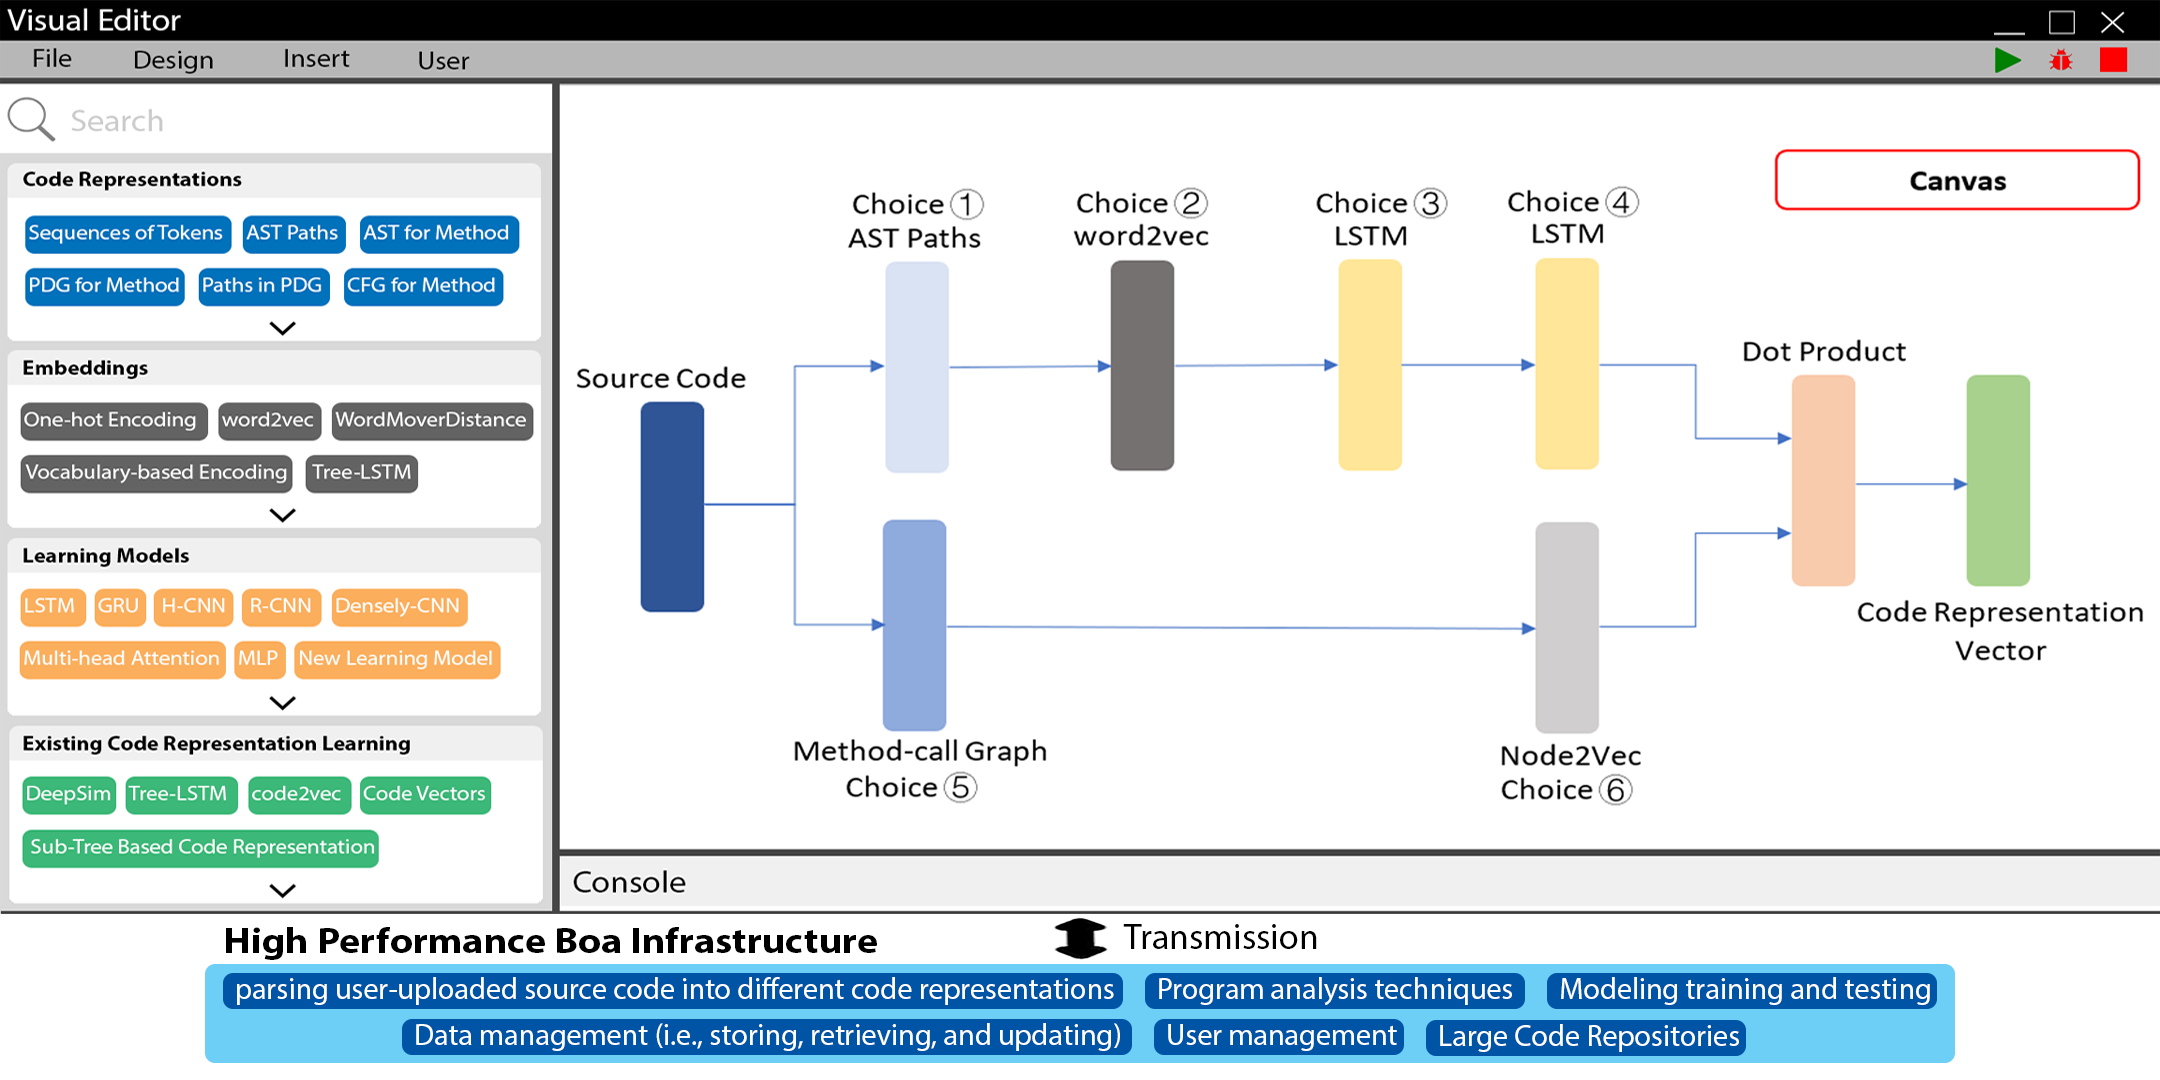
\includegraphics[scale=0.16]{graphs/editor.png}
	\vspace{-15pt}
	\caption{Design Environment for CRL}
	\label{editor}
	\vspace{-10pt}
\end{wrapfigure}

\underline{\textit{(3) Learning Models:}} shows a list of learning
models taking the embeddings of code representations (CRs) as inputs
and learn to generate vectors to represent the CRs, such as the ones
in the row ``Learning Models'' of Table~\ref{framework} and even
user-built models (as long as using tenserflow APIs).
\underline{\textit{(4) Existing Code Representation Learning (CRL):}}
show a list of existing CRL approaches that have been pre-built and
pre-run on our back-end system.  \underline{(5) \textit{Canvas:}}
Users can drag-and-drop code representations, embeddings, models, and
existing CRL approaches onto the canvas to streamline a workflow of a
CRL approach.  \underline{(6) \textit{Tool Bar and Runtime Tools:}}
\textit{Tool Bar} contains file basic functions, such as
start/save/edit/open a project/workflow, upload source
code. \textit{Runtime Tools:} Once a workflow is saved, users can run
the defined workflow and see/save the results (i.e., vectors) to a
local file system.  \underline{\textit{(7) Search Bar and
    Console}}. Users can search relevant code representations,
embedding, learning models and existing CRL approaches in Search
Bar. \textit{Console} shows messages, e.g., run-time and design
errors, and warnings.  \textit{User Accounts:} managing user
information.


\subsection{T1 Task 3. Plan-to-Do: Scalable Program Analysis for Effective Code Representations via Boa}

We build our editor on top of
Boa~\cite{boa,Dyer-Nguyen-Rajan-Nguyen-13}
%, a high-performance
%ultra-large infrastructure,
in which PI Nguyen is the co-founder.
%widely used in SE and PA research. PI Nguyen is the co-founder of Boa
%and we have the full access to Boa. Leveraging Boa's existing power,
Boa will provide the following key functions to our editor: parsing
source code, program analysis techniques, modeling training and
testing, large-scale data processing. Boa brings the scalable program
analysis and effectiveness in producing high-quality vector
representations with ultra-large training data.
%
First, a user uses Boa editor to write a query to perform program
analysis on the code under study.
%to produce the data structures required for the bug detect-fix task.
%
%Figure~\ref{fig:boa} shows an example of using Boa to traverse the CFG
%of a project in a forward, depth-first search fashion and collect the
%names of the nodes in the CFG.
In general, Boa supports any types of custom traversal for any program
analyses including the standard data structures (AST, CFG, DFG,
PDG). The results from the Program Analysis from Boa will be fed into
the visual editor (Task 2).  Then, the user continues editing to
construct the DL model for CRL on the data produced by Boa as part of
the traversal.

%Tien
%\begin{wrapfigure}{r}{0.625\textwidth}
%	\vspace{-10pt}
%	\centering
%	\renewcommand{\lstlistingname}{Method}
%	\lstset{
%		numbers=left,
%		numberstyle= \tiny,
%		keywordstyle= \color{blue!70},
%		commentstyle= \color{red!50!green!50!blue!50},
%		frame=shadowbox,
%		rulesepcolor= \color{red!20!green!20!blue!20} ,
%		xleftmargin=1em,xrightmargin=0em, aboveskip=1em,
%		framexleftmargin=1em,
%		language=Java,
%		basicstyle=\footnotesize,
 %               moredelim=**[is][\color{red}]{@}{@},
%		escapeinside= {(*@}{@*)}
%	}
%	\begin{lstlisting}
 % ids: output collection of string;
%  printNodes := traversal(n: CFGNode) {
%      ids << n.name;
%  };
%  visit(input, visitor {
%      before m: Method -> {
%          cfg := getCFG(m);
%          traverse(cfg, TraversalDirection.FW, Traversal.DFS, printNodes);
%      }
%      after: m: Method {
%         editor.invoke (ids);
%      }
%  });
%\end{lstlisting}
%\vspace{-0.10in}
%\caption{Program Analysis in Boa for Large-scale Code Representation Learning}
%  \label{fig:boa}
%\vspace{-10pt}
%\end{wrapfigure}



%The visual editor has the following main features: (1) It reminds
%users with design conflicts and obvious design errors, e.g., it is
%unorthodox to combine a vector learned from a path in an AST and
%another vector learned from a method, as these two vectors model the
%information at different levels.  (2) Users can drag-and-drop
%predefined building blocks into a drawing canvas to design their own
%code representation approach as a workflow of building blocks; (3)
%Users can view, edit, update, and replace any block within a workflow
%on the canvas; (4) When users drag-and-drop an existing CRL approach
%onto the canvas, the CRL approach can be unfolded into a workflow and
%composed with other building blocks; (5) Users can upload their own
%code representations, embeddings, models onto Boa through our editor
%and design their workflows.


\textbf{An example of use case of our editor as drawn on the canvas in
  Figure~\ref{editor}}.  A user
writes a Boa query to perform program analysis to produce the results,
e.g., the ASTs. The ASTs of the projects under study are fed into our
editor and the user graphically designs their CRL. At
\textbf{C\circled{1}}, the user can drag-and-drop AST Paths icon from
the \textit{Code Representations} onto the canvas.  Then, the user can
choose \textit{word2vec} from the \textit{Embeddings} at
\textbf{C\circled{2}} to convert all AST nodes of a path into vectors.
At \textbf{C\circled{3}}, the user can add a LSTM model on the ordered
list of node vectors to combine all AST node vectors to generate only
one vector for a path. At \textbf{C\circled{4}}, the user can choose
the same LSTM model on a bag of path vectors to learn one vector for a
method.  To model relations among methods, the user can use a
method-call graph to model the relations at \textbf{C\circled{5}}. In
the graph, each node is a method, the user can choose Node2Vec, to
encode each node at \textbf{C\circled{6}}. Now, a method has two
vectors: one learned from the method body (through
\textbf{C\circled{1}}, \textbf{C\circled{2}}, \textbf{C\circled{3}},
and \textbf{C\circled{4})} and another one learned from the relations
between a method and its neighboring nodes. To generate a method
vector with both types of information, the user can choose
\textit{dot product} to combine the above two methods.

%Last, we can run a classification model on the top of the generated method vectors to train a classification model to judge whether a given method buggy or non-buggy.

%A user can use simple drag-and-drops of building blocks to implement their ideas of code representation learning. After the design, the user can actually run the workflow inside our editor and generate code vectors for software engineering/program analysis tasks. The user can also quickly adjust choices at each design choice to test a new idea. Importantly, our editor will generate warnings/errors/recommendations based on our empirical results to users based on their current and previous choices. For example, to combine an ordered list of vectors from the same type of information, LSTM can work well. However, it is not a good idea to run LSTM on the top of vectors from distinct information sources. 
